\qns{Transistor Switch Model}
\qcontributor{Ryan Koh}
\qcontributor{Son Tran}

You have two CMOS inverters made from NMOS and PMOS devices. Both NMOS and PMOS devices have an "on resistance" of $R_{on}=\SI{1}{\kilo\ohm}$, and each has a gate capacitance (input capacitance) of $C=\SI{1}{\femto\farad}$ (femto-Farads = $10^{-15}$).
We assume the "off resistance" (the resistance when the transistor is off) is infinite (i.e., the transistor acts as an open circuit when off).
The supply voltage $V_{DD}$ is $\SI{1}{\volt}$. The two inverters are connected in series, with the output of the first inverter driving the input of the second inverter.

  \begin{figure}[H]
  \begin{center}
    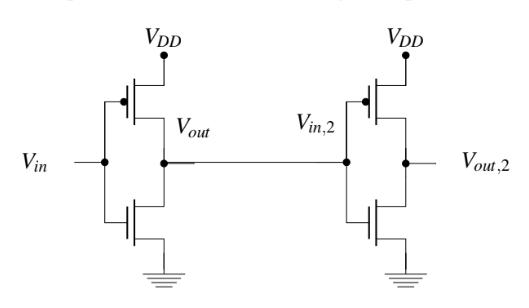
\includegraphics[width=0.6\linewidth]{\bank/ode/figures/transwitchmodel_cmos.png}
  \end{center}
  \label{fig:cmos}
\end{figure}




\begin{enumerate}



% Part (a)
\qitem Assume the input to the first inverter has been low ($V_{in} = \SI{0}{\volt}$) for a long time, and then switches at time $t = 0$ to high ($V_{in} = V_{DD}$).
\textbf{Draw a simple RC circuit and write a differential equation describing the output voltage of the first inverter for time $t \geq 0$}.
Don’t forget that the second inverter is "loading" the output of the first inverter - you need to think about both of them.

\sol {
  The input to the first inverter was low for a long time.
  This means the output of the inverter had been held at high for a long time.
  To analyze this circuit as an RC circuit we can recall the transistor switch model.
  Using this we can see that the first inverter’s output appears as a resistor connected to $V_{DD}$ when the input is low or a resistor connected to ground when the input turns high.
  \\
  \\
  The second inverter "loads" the output of the first inverter.
  Modeling the gates of the transistors as capacitors, these gates together form our capacitive load.
  The gate of the PMOS acts as a capacitor to $V_{dd}$ and the gate of the NMOS acts as a capacitor to ground.
  \\
  \\
  We can then draw the following RC circuit:

  \begin{figure}[H]
  \begin{center}
    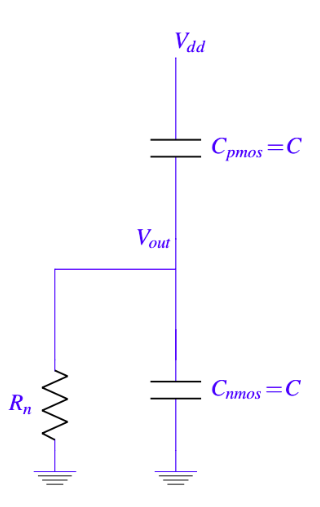
\includegraphics[width=0.4\linewidth]{\bank/ode/figures/transwitchmodel_first_inverter.png}
  \end{center}
  \label{fig:inverter0}
\end{figure}


  To get the differential equation describing the output of the first inverter at time $t \geq 0$ let us first think about the behavior of the circuit at and after $t = 0$.

  At $t = 0$ we know that the output $V_{out} = V_{dd}$.
  This means that $C_{nmos}$ is charged while the $C_{pmos}$ is not as there is no voltage difference across it.
  When the input to the inverter changes the output goes to zero in steady state.
  \\
  \\
  For this to occur the $C_{pmos}$ must start discharging and $C_{nmos}$ must start charging to $V_{dd}$.
  We know the voltage across $C_{pmos}$ is $V_{out}(t) - V_{dd}$ and the voltage across $C_{nmos}$ is $V_{out}(t)$.
  Using this information we can set up a differential equation to solve for $V_{out}(t)$:

\begin{align*}
  I_{c_{pmos}} = C_{pmos} \frac{d}{dt}(V_{out}(t) - V_{dd}) \\
  I_{c_{nmos}} = C_{nmos} \frac{d}{dt}V_{out}(t) \\
  I_{R_{on}} = \frac{V_{out}(t)}{R_{on}} \\
  I_{c_{pmos}} + I_{c_{nmos}} = -I_{R_{on}} \\
  C_{pmos} \frac {d}{dt} (V_{out}(t) - V_{dd}) + C_{nmos} \frac {d}{dt} V_{out}(t) = - \frac {V_{out}(t)}{R_{on}} \\
  C_{pmos} \frac {d}{dt} V_{out}(t) + C_{nmos} \frac{d}{dt} V_{out}(t) = - \frac {V_{out} (t)} {R_{on}} \\
  (C_{pmos} + C_{nmos}) \frac {d}{dt} V_{out} (t) = - \frac {V_{out}(t)} {R_{on}} \\
  \frac {d}{dt} V_{out}(t) = - \frac {V_{out} (t)} {R_{on} (C_{pmos} + C_{nmos})} \\
  \frac {d}{dt} V_{out} (t) = - \frac {V_{out} (t)} {R_{on} (2C)}
\end{align*}
}



% Part (b)
\qitem \textbf{Sketch the output voltage of the first inverter, showing clearly (1) the initial value, (2) the initial slope, (3) the asymptotic value, and (4) the time that it takes for the voltage to decay to roughly $\mathbf{\frac{1}{3}}$ of its initial value.}

\sol{
  (1) We know that the output of our inverter started with the initial value $V_{dd}$.
  \\
  \\
  (2) Since the differential equation tells us the change in value of $V_{out}(t)$ at time $t$ we can simply plug in $t = 0$ into our differential equation to get the initial slope:

  \begin{align*}
    \frac{d}{dt}V_{out}(t) = - \frac{V_{out}(0)}{R_{on}(C_{nmos} + C_{pmos})} \\
    \frac{d}{dt}V_{out}(t) = - \frac{V_{dd}}{R_{on}(C_{nmos} + C_{pmos})}
  \end{align*}

  Thus the initial slope is $\frac{V_{dd}}{R_{on}(C_{nmos} + C_{pmos})} = \frac{V_{dd}}{R_{on}(2C)}$
  \\
  \\
  (3) Since the input to the inverter changed from high to low we know the output of the inverter is going to go to $0$ in steady state.
  \\
  \\
  Another way to find this is: We know that the solution to a differential equation of the form $\frac{d}{dt}V_{out}(t) = - \frac{V_{out}}{R_{on}(C_{nmos} + C_{pmos})}$ is $V_{out} = ke^{-\frac{t}{R_{on}(2C)}}$.
  Plugging in the initial condition $V_{out}(0) = V_{dd}$ we find that $V_{out} = V_{dd}e^{-\frac{t}{R_{on}(2C)}}$.
  \\
  \\
  Plugging in $t = \infty$ we can see that the output approaches $V_{out} = V_{dd}e^{-\frac{\infty}{R_{on}(2C)}} = 0$.

  \begin{figure}[H]
  \begin{center}
    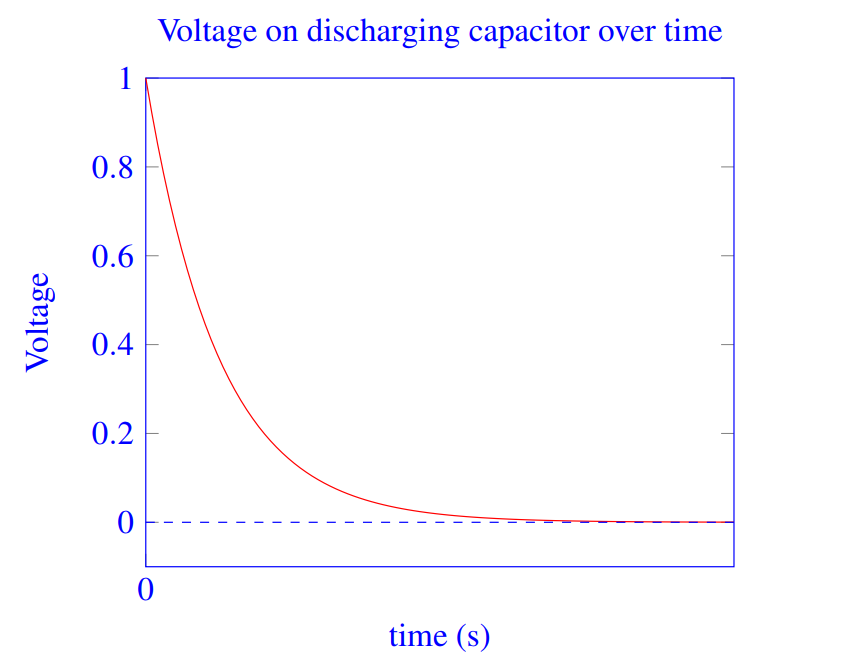
\includegraphics[width=0.6\linewidth]{\bank/ode/figures/discharging_capacitor.png}
  \end{center}
  \label{fig:discharging_capacitor}
\end{figure}


  (4) Using the fact that $e^{-1} = \frac{1}{e} \approx \frac{1}{3}$, we know that $V_{out} = V_{dd}e^{-1}$ which occurs when $t = R_{on}(2C) = 2 * 10^{-12}$.

  We know this from the solution $V_{out} = V_{dd}e^{-\frac{t}{R_{on}(2C)}}$ of the differential equation that we derived found in the previous part.
}




% Part (c)
\qitem A long time later, the input to the first inverter switches low again.
\textbf{Sketch the output voltage of the first inverter, showing clearly (1) the initial value, (2) the initial slope, and (3) the asymptotic value.}

\sol{
After a long time we know that the output of the first inverter has stabilized to 0.
When we switch the input of the first inverter back to low again, we know that the output will move towards $V_{dd}$.
Using this we establish that:
\\
\\
(1) The initial value of $V_{out}(t) = 0$
\\
\\
(2) When the input to the inverter has flipped to low the RC circuit is:

  \begin{figure}[H]
  \begin{center}
    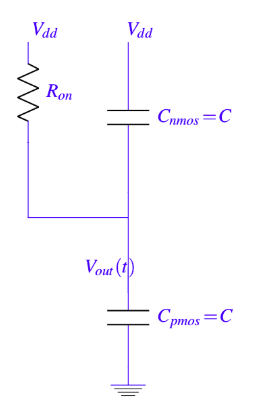
\includegraphics[width=0.3\linewidth]{\bank/ode/figures/transwitchmodel_second_inverter.png}
  \end{center}
  \label{fig:inverter1}
\end{figure}


$V_{out}$ was 0 to start with and is slowly changing to $V_{dd}$.
Due to this we know that $C_{pmos}$ is slowly discharging as the voltage across it drops to 0 and $C_{nmos}$ is slowly charging as the voltage across it increases to $V_{dd}$.
Using this information we get the following:

\begin{align*}
  I_{C_{pmos}} = C_{pmos} \frac{d}{dt}(V_{out}(t) - V_{dd}) \\
  I_{C_{nmos}} = C_{nmos} \frac{d}{dt}V_{out}(t) \\
  I_{R_{on}} = \frac{V_{out}(t) - V_{dd}}{R_{on}} \\
  I_{c_{pmos}} + I_{c_{nmos}} = -I_{R_{on}} \\
  C_{pmos} \frac {d}{dt} (V_{out}(t) - V_{dd}) + C_{nmos} \frac {d}{dt} V_{out}(t) = - \frac {V_{out}(t) - V_{dd}}{R_{on}} \\
  C_{pmos} \frac {d}{dt} V_{out}(t) + C_{nmos} \frac{d}{dt} V_{out}(t) = - \frac {V_{out} (t) - V_{dd}} {R_{on}} \\
  (C_{pmos} + C_{nmos}) \frac {d}{dt} V_{out} (t) = - \frac {V_{out}(t) - V_{d}} {R_{on}} \\
  \frac {d}{dt} V_{out}(t) = \frac {V_{dd} - V_{out} (t)} {R_{on} (C_{pmos} + C_{nmos})} \\
  \frac {d}{dt} V_{out} (t) = \frac {V_{dd} - V_{out} (t)} {R_{on} (2C)} \\
\end{align*}

To find the initial value of the slope we can plug in zero to the above differential equation: $\frac {d}{dt} V_{out} (t) = \frac {(V_{dd} - V_{out} (0))}{R_{on} (2C)}$ where $V_{out} (0) = 0$.
Thus our initial slope is $\frac {V_{dd}} {R_{on} (2C)}$.
\\
\\
(3) Since the input to the inverter changed from low to high, we know the output of the inverter is going to go to $V_{dd}$ in steady state.
\\
\\
The differential equation we derived above is just like the equation for a capacitor charging up to $V_{dd}$ through a resistor $R_{on}$ and capacitor where $C = 2C$.
Recall that the solution to this differential equation is: $V_{out}(t) = V_{dd}(1 - e^{- \frac {t}{R_{on} (2C)}})$.
Plugging in $t = \infty$ we can see that the value of $V_{out}(t)$ approaches $V_{dd}$.

  \begin{figure}[H]
  \begin{center}
    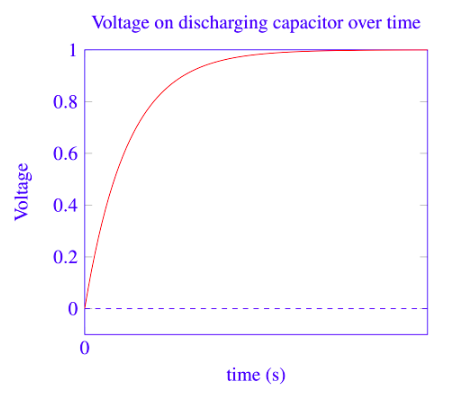
\includegraphics[width=0.6\linewidth]{\bank/ode/figures/transwitchmodel_dischargingC.png}
  \end{center}
  \label{fig:discharging_capacitor}
\end{figure}

}


% Part (d)
\qitem For each complete input cycle described in the two steps above, \textbf{how much charge is pulled out of the power supply?}
Give both a symbolic and numerical answer.

\sol{
  We can see that for each stage of the input cycle one of the gate capacitors charges up and the other discharges.
  The power supply only supplies charge to charge up a gate capacitor.
  Using $Q = CV$ we now that the voltage suplly outpus $Q = 10^{-15}*1$ at each step of the cycle.
  So for the total charge outputted for each complete input cycle is $Q = 2*10^{-15}$.
}

\end{enumerate}
